\chapter{Efficient optimization of sparsity and smoothness regularized models}\label{chap:efficient_opt}
\markright{{~{\rm \ref{chap:efficient_opt}}. Algorithms for structured priors}\hfill}{}
\newthought{Though the SpaceNet model} presented above leads to superior estimators compared to classical estimators (Ridge regression, SVM, etc.) without spatial penalization, it is considerably harder to optimize than these classical models. Indeed, the corresponding optimization problems is non-separable in the model coefficients, and except for the case of GraphNet~\citep{hebiri2011,grosenick2013} and social-sparsity~\citep{kowalski2013social,varoquaux2016social},
the penalty term $\mathcal P(\w)$ is neither smooth nor proximable.
\footnote{ A function $f$ is said to be \textit{proximable} is the operator $\text{prox}_{\gamma f}$ is easy to compute. This is the case for $\ell_p$-norms  (with $ p \ge 1$, to ensure convexity) and indicator functions of simple closed convex sets like balls, simplexes, half-spaces, etc.}
For the penalty to fully exercise its
structuring effect on the maps, this optimization problem must be
solved to a good tolerance resulting in a computational challenge. Lack of good solver and explicit control of
tolerance can lead to brain maps and conclusions that reflect
properties of the solver more than of model coefficients, as illustrated in Fig. \ref{Fig:benchmarks_prni}.

  %% \begin{itemize}
  %% \item{proximal methods}
  %%   \begin{itemize}
  %%     \item single-step\\
  %%       {-} ISTA (Iterative Soft-Thresholding Algorithm)   \citep{daubechies2004}
  %%     \item multi-step / accelerated\\
  %%       {-} FISTA (Fast ISTA)   \citep{beck09fista}
  %%   \end{itemize}
  %% \item {primal-dual \& splitting methods}
  %%   \begin{itemize}
  %%   \item ADMM (Alternating Directions Method of Multipliers)   \citep{boyd2011distributed}
  %%     % (\textit{Alternating Directions Method of Multipliers})
  %%   \item Chambolle-Pock's Primal-Dual   \citep{chambolle2010}
  %%   \end{itemize}
  %% \item {quasi-Newton methods}
  %%   \begin{itemize}
  %%   \item HANSO ({Hybrid Algorithm for Non-smooth Optimization})   \citep{lewis2008}
  %%   \item L-BFGS   \citep{ciyou1994} on smooth surrogates of the penalty
  %%   \end{itemize}
  %% \end{itemize}
  

%% \begin{figure*}
%%   \begin{subfigure}[t]{1\linewidth}
%%     \hspace*{-.01\linewidth}%
%%     \includegraphics[width=.6\linewidth]{haxby_lr_energy.pdf}
%%     \hspace*{-.09\linewidth}%
%%     \includegraphics[width=.6\linewidth]{haxby_lr.pdf}%
%%     % \vspace{-2ex}
%%     \caption{\textbf{Classification} with logistic regression model
%%       \eqref{eq:opt_pb}. on the visual recognition face-house
%%     discrimination task. \textbf{Left}: excess energy $E(\mathbf{w}_t) -
%%     E(\mathbf{w})_{t \rightarrow \infty}$ as a function 
%%     of time.
%%     \textbf{Right}: convergence time of the various solvers for different
%%     choice of regularization parameters.
%%     Broken lines correspond to a tolerance of $10^{0}$,
%%     whilst full-lines correspond to $10^{-2}$.  The thick vertical line
%%     indicates the best model selected by cross-validation.}
%%     \label{Fig:HaxbyLR}
%%   \end{subfigure}
%%   \begin{subfigure}[t]{1\linewidth}
%%     \includegraphics[width=.6\linewidth]{haxby_mse.pdf}%
%%     \hspace{-.09\linewidth}%
%%     % generate with: ipython ../wip/tv_l1_solver/plot_parallel_plots.py poldrack_mse_12th.json 2e1 --pdb
%%     \includegraphics[width=.6\linewidth]{poldrack_mse.pdf}
%%     % \vspace{-2ex}
%%     \caption{\textbf{Regression.} results. \textbf{Left}:
%%       on the visual recognition  face-house discrimination task; \textbf{Right}: on the
%%       Mixed gambles dataset. Broken lines correspond to a tolerance of $10^{0}$,
%%       whilst full-lines correspond to $10^{-2}$. The thick vertical line
%%       indicates the best model selected by cross-validation.}
%%     \label{Fig:MSEtimes}
%%   \end{subfigure}
%% \caption{Benchmarks for different solvers for the TV-$\ell_1$ model
%%   \eqref{eq:opt_pb} on the visual recognition face-house
%%   discrimination task. See   \citep{dohmatob2014benchmarking} for more details.}
%% \end{figure*}

\section{Solving TV-L1 regularized problems}
\begin{figure}[!htb]
    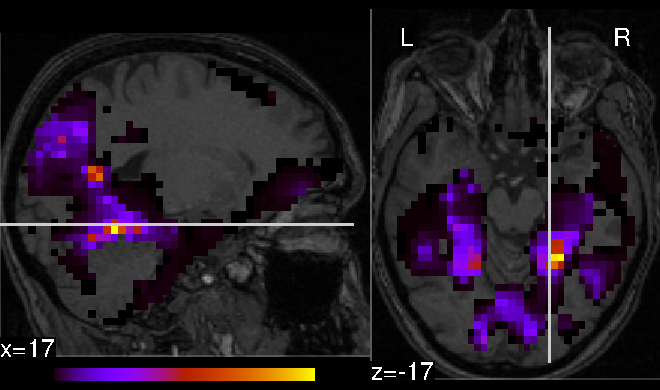
\includegraphics[width=.331\linewidth]{face_vs_house_tol_0_1.pdf}%
\llap{\color{white}\raisebox{.17\linewidth}{\rlap{\sffamily Stopping:
      $\Delta E < 10^{-1}$}}\hspace*{.315\linewidth}}\hfill%
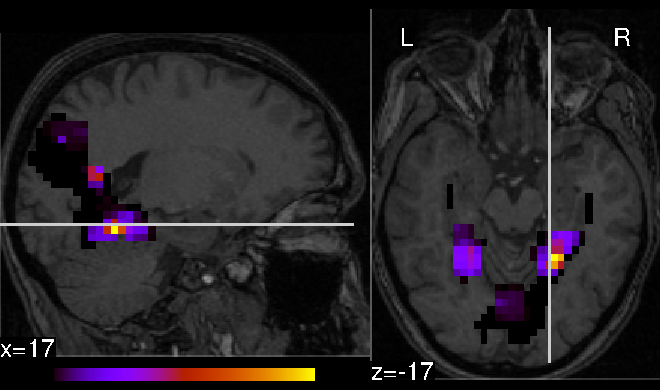
\includegraphics[width=.331\linewidth]{face_vs_house_tol_0_001.pdf}%
\llap{\color{white}\raisebox{.17\linewidth}{\rlap{\sffamily Stopping:
      $\Delta E < 10^{-3}$}}\hspace*{.315\linewidth}}\hfill%
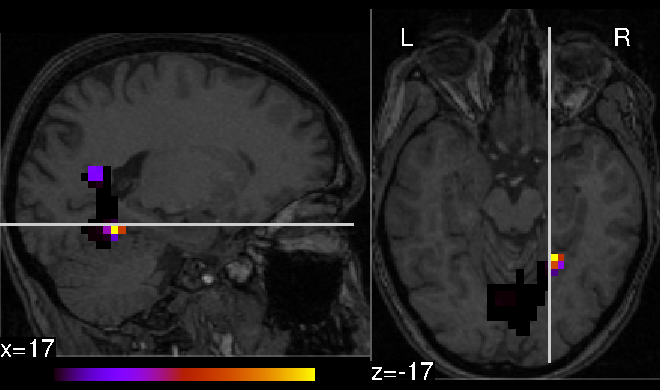
\includegraphics[width=.331\linewidth]{face_vs_house_tol_1e-05.pdf}%
\llap{\color{white}\raisebox{.17\linewidth}{\rlap{\sffamily Stopping:
      $\Delta E < 10^{-5}$}}\hspace*{.315\linewidth}}%

\caption{TV-$\ell_1$ maps for the face-house discrimination task on
  the visual recognition dataset.
  Note that
  the stopping criterion is defined as a threshold on the energy
  decrease per one iteration of the algorithm, and thus differs from
  the tolerance displayed in figure \ref{Fig:benchmarks_prni}.  This figure shows
  the importance of convergence for problem \eqref{eq:opt_pb}, and motivates
  the need for fast solvers for SpaceNet priors, especially the non-smooth ones like TV-$\ell_1$ and Sparse Variation. See the full story in
  \citep{dohmatob2014benchmarking}}
  \label{Fig:benchmarks_prni}
\end{figure}
The optimization problem \eqref{eq:opt_pb} is very challenging:
it is non-smooth (except in the case of Laplacian regularization), non-separable and heavily ill-conditioned. For the penalty to fully exercise its
structuring effect on the maps, this optimization problem must be
solved to a good tolerance resulting in a computational challenge.
In \citep{dohmatob2014benchmarking}, we did an extensive study of all solvers applicable to the problem in TV-$\ell_1$ special case (which happens to be the most difficult scenario).
Our results outlined the best strategy: a double FISTA loop, where the
inner loop computes the proximal operator of the penalty term, with approximate precision on the duality-gap. This was further refined and implemented in   \citep{varoquaux2015faasta}.

% In  \citep{dohmatob2014benchmarking}, we explored a wide variety of solvers and exhibited their
% convergence properties on fMRI data. Below we present a brief overview of the paper.

\subsection{The algorithms}
\paragraph{ISTA/FISTA.}
ISTA~ \citep{daubechies2004}, and its accelerated variant
FISTA~ \citep{beck2009a}, are proximal gradient approaches: the go-to
methods for non-smooth optimization. In their seminal introduction of TV
for fMRI,  \citep{michel2011} relied on ISTA.
The challenge of these methods for TV is that the proximal operator
%% \footnote{The proximal operator (or prox for short) can be seen as a generalization of projection unto convex set.}
  of TV
cannot be computed exactly; we approximate it in an inner FISTA loop
 \citep{beck2009b,michel2011}.
% ,  \citep{gramfort-etal:2013a}.
%%  and must itself be solved by a
%% FISTA\footnote{Note that solving TV and TV$-\ell_1$ are formally very
%% close  \citep{gramfort-etal:2013a}.
% }
%  \citep{beck2009b,michel2011}. 
Here, for all FISTA implementations we use
the faster monotonous FISTA variant  \citep{beck2009b}. We control the
optimality of the TV proximal via its dual gap  \citep{michel2011} and
use a line-search strategy in the monotonous FISTA to decrease the
tolerance as the algorithm progresses, ensuring convergence of the
TV-$\ell_1$ regression with good accuracy.

\paragraph{ISTA/FISTA with backtracking.}
A key ingredient in FISTA's convergence is the Lipschitz
constant $L_{\nabla \ell}$, of the derivative of smooth part of the objective function
. The tighter the upper bound used for this constant,
the faster the resulting FISTA algorithm. In FISTA, the main use of 
$L_{\nabla \ell}$ is the fact that: for any
stepsize $0 < t \le 1/L_{\nabla \ell}$ and for any point $\mathbf{z}$,
\begin{equation}%
  \begin{gathered}
    \ell(\mathbf{p}_{t}(\mathbf{z})) \le
    \ell(\mathbf{z}) + \mathbf{r}_{t}^T\nabla
    \ell(\mathbf{z}) + \frac{1}{2t} \|\mathbf{r}_{t}\|_{2}^2,
    \text{  where} \quad\\
    \mathbf{p}_{t}(\mathbf{z}) := \textrm{prox}_{\alpha t J}(\mathbf{z} - t
    \nabla \ell(\mathbf{z})) \,\text{  and  }\,
    \mathbf{r}_{t} :=
    \mathbf{p}_{t}(\mathbf{z}) - \mathbf{z} \quad
  \end{gathered}
  \label{eq:fista_ineq}
\end{equation}
In least-squares regression, $L_{\nabla \ell}$ is precisely the largest
singular value of the design matrix $\mathbf{X}$.
For logistic
regression however, the tightest known upper bound for
$L_{\nabla \ell}$ is $\|\mathbf{X}\|\|\mathbf{X}^T\|$,
% (for example see Appendix A of  \citep{yuan2012}),
which performs very poorly locally (i.e, stepsizes $\sim 1 / L_{\nabla \ell}$ are
sub-optimal locally). A way to circumvent this difficulty is
\emph{backtracking line search}  \citep{beck2009a}, where one tunes the
stepsize $t$ to satisfy inequality \eqref{eq:fista_ineq} locally at
point $\mathbf{z}$. 


\paragraph{ADMM: Alternating Direction Method of Multipliers.}
ADMM is a Bregman Operator Splitting primal-dual method for
solving convex-optimization problems by splitting the
objective function in two convex terms which are functions of linearly-related auxiliary variables
 \citep{boyd2010}.  ADMM is particularly appealing for problems such as TV
regression: using the variable split $\mathbf{z}
\leftarrow \nabla \mathbf{w}$, the regularization is a simple $\ell_{1}/\ell_2$
norm on $\mathbf{z}$ for which the proximal is exact and computationally
cheap. However, in our settings, limitations of ADMM are:
\begin{itemize}
\item The $\mathbf{w}$-update involves the inversion of a large $p$-by-$p$
  ill-conditioned linear operator (precisely a weighted sum of
  $\mathbf{X}^T\mathbf{X}$, the laplacian $\Delta$, and the identity
  operator).
\item The $\rho$ parameter for penalizing the split
  residual $\mathbf{z} - \nabla \mathbf{w}$ is hard to set (this is still an
  open problem), and though under mild conditions ADMM
  converges for any value of $\rho$, the convergence rate depends
  on $\rho$.
\end{itemize}

\paragraph{Primal-Dual algorithm of Chambolle and Pock  \citep{chambolle2010}.}
this scheme is another method based on operator splitting.
Used for fMRI TV regression by  \citep{gramfort-etal:2013a},
it does not require setting a hyperparameter.  % XXX : this is wrong you have the tau / sigma
However it is a first-order single-step method and is thus more impacted by the
conditioning of the problem. Note that here we explore this primal-dual
method only in the squared loss setting, in which the algorithm can be accelerated by
precomputing the SVD of $\mathbf{X}$  \citep{gramfort-etal:2013a}
.

\paragraph{HANSO  \citep{lewis2008}.}
a modified LBFGS scheme based on gradient 
sampling methods  \citep{burke2005} and inexact
line-search. For non-smooth problems as in our case, the algorithm relies on
random initialization, to avoid singularities with high probability. 
Here, we used the original authors' implementation.

\paragraph{Uniform approximation by smooth convex surrogates.}
The $\ell_{1}$ norm (resp. TV semi-norm) is differentiable everywhere with
gradient $\left(w_j/|w_j|\right)_{j \in [\![p]\!]}$ (resp. $-\dive (((\nabla \mathbf{w})_j/\|(\nabla \mathbf{w})_j\|_2)_{j \in [\![p]\!]}))$), except when some voxels are inactive with
$w_j = 0$ (resp. $(\nabla \w)_j = 0$), corresponding to black spots (resp. edges).  A convenient
approach (see for example  \citep{NESTA, nesterov2005a, nesterov2005b,
  beck2012}) for dealing with such singularities is to uniformly
approximate the offending function with smooth surrogates that
preserve its convexity. Given  % I removed "and other important properties"
a smoothing parameter $\mu > 0$, we define \emph{smoothed} versions
of $\ell_1$ and TV:
%
\begin{eqnarray}
    \|\mathbf{w}\|_{1,\mu} := \sum_j
    \sqrt{\mathbf{w}_j^2 + \mu^2},\;
    \|\mathbf{w}\|_{\text{TV}, \mu} :=
    \sum_{j} \sqrt{\|\nabla \mathbf{w}_j\|_{2}^2 + \mu^2}
\end{eqnarray}
These surrogate upper-bounds are convex and everywhere-differentiable
with gradients that are Lipschitz-continuous with constants $1/\mu$ and
$\|\nabla\|^2(1/\mu) = 12 / \mu$ respectively.
They lead to smoothed versions of problem \eqref{eq:opt_pb}:
\begin{align}
  \mathbf{\hat{w}}_{\mu} := \argmin_{\mathbf{w}}\;
  \{E_{\mu}(\mathbf{w}) := \ell(\mathbf{w}) + \alpha
    \mathcal P_{\text{TV-L1},\mu}(\mathbf{w})\},
  \label{eq:sopt_pb}
\end{align}
where    $\mathcal P_{\text{TV-L1},\mu}(\mathbf{w}) :=\rho \|\mathbf{w}\|_{1,\mu} +
(1 - \rho)\|\mathbf{w}\|_{\text{TV}, \mu}$.

To solve \eqref{eq:opt_pb}, we consider problems of the form
\eqref{eq:sopt_pb} with $\mu \rightarrow 0^+$: we start with a coarse
$\mu$ ($= 10^{-2}$, \emph{e.g}) and cheaply solve the $\mu$-smoothed problem
\eqref{eq:sopt_pb} to a precision $\sim \mu$ using a fast
iterative oracle like the LBFGS \citep{ciyou1994}; we
obtain a better estimate for the solution; then we decrease $\mu$ by a fixed factor,
and restart the solver on problem \eqref{eq:sopt_pb} with this solution; and so on, in a 
\emph{continuation} process~\citep{NESTA} detailed in Alg.
\ref{Tab:pseudocode_lbfgs}.
This algorithm is not faster than
$\mathcal{O}(1/\epsilon)$: indeed a good optimization algorithm
for the sub-problem \eqref{eq:sopt_pb} is $\mathcal{O}(\sqrt{L_{\mu}/\epsilon})$
\citep{nesterov1983}, and $L_{\mu} \sim 1 / \mu \sim 1 / \epsilon$. We
believe that this bound is tight but a detailed analysis is
beyond the scope of this paper.
\begin{algorithm}
  \caption{LBFGS algorithm with continuation}
  \label{Tab:pseudocode_lbfgs}  
  \begin{algorithmic}[1]  
    \Require $\epsilon > 0$ the desired precision, $\beta$ ($0 < \beta <
    1$) the rate of decay of the smoothing parameter $\mu$, and $\gamma > 0$ be a constant.
    Finally,
    let LBFGS: $(E_\mu, \mathbf{w}^{(0)}, \epsilon) \mapsto \mathbf{w}$ be
    an oracle which when warm-started with an initial guess
    $\mathbf{w}^{(0)}$, returns an $\epsilon$-optimal
    solution (i.e $E_\mu(\mathbf{w}) - E_\mu^{*} < \epsilon$) for problem \eqref{eq:sopt_pb}.\\
    \textbf{Initialize} $ 0 < \mu^{(0)}$ ($= 10^{-2}$, \emph{e.g}),
    $\mathbf{w}^{(0)}\in \mathbb{R}^p$, and $k = 0$.
    \While{$\gamma\mu^{(k)} \ge \epsilon$}
    \State $\mathbf{w}^{(k + 1)} \leftarrow \mbox{LBFGS}(E_{\mu^{(k)}}, \mathbf{w}^{(k)}, \gamma\mu^{(k)})$
    \State $\mu^{(k + 1)} \leftarrow \beta \mu^{(k)}$
    \State $k \leftarrow k + 1$
    \EndWhile
  \end{algorithmic}
\end{algorithm}

\subsection{Experiments on fMRI datasets}
\label{sec:experiments}
We now detail experiments done on publicly available
data. All experiments were run full-brain without spatial smoothing.

\paragraph{Visual recognition.}
\label{subsec:haxby}
Our first benchmark dataset is a popular block-design fMRI dataset from a study on face and
object representation in human ventral temporal cortex  \citep{haxby2001}.
It consists of
6 subjects with 12 runs per subject. In each run, the subjects
passively viewed images of eight object categories, grouped
in 24-second blocks separated by intermittent rest periods. This
experiment is a classification task: predicting the object category. We use a
two-class prediction target: $\mathbf{y}$ encodes faces versus houses.
The design matrix $\mathbf{X}$ is made of
time-series from the full-brain mask of $p = 23\,707$ voxels over $n =
216$ TRs, of a single subject (subj1).

\paragraph{Mixed Gambles.}
Our second benchmark dataset is a study in which
subjects were presented with mixed (gain/loss) gambles, and decided
whether they would accept each gamble \citep{mixedgambles2007}.  No outcomes of these gambles
were presented during scanning, but after the scan three gambles were
elected at random and played for real money. The prediction task here is
to predict the magnitude of the gain and thus a regression on a
continuous variable \citep{jimura2012}. The data is pooled across
subjects, resulting in 768 samples, each an image of 33\,177 voxels.

% We validate our algorithms on both simulated and real data.
\smallskip

We study the convergence of the algorithms for parameters close to the
optimal parameters set by 10-fold cross-validation to maximize prediction
accuracy.

\subsection{Results: convergence times}
 \begin{figure}[!htbp]
   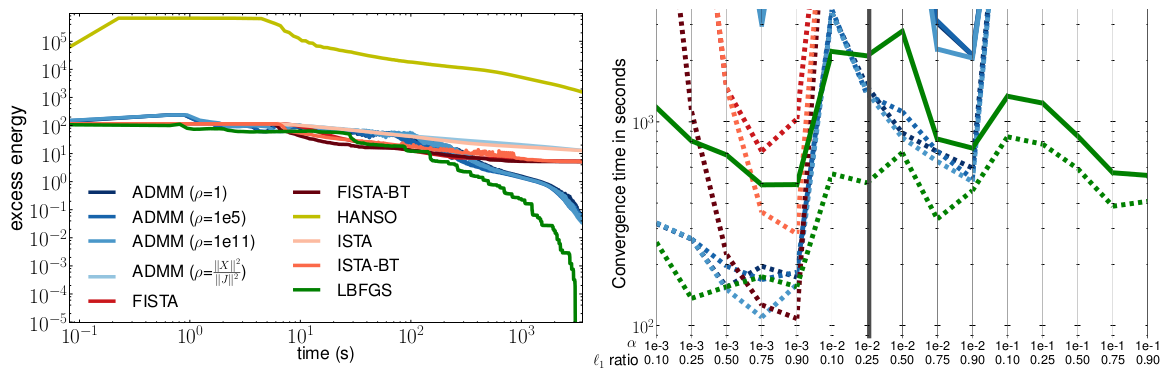
\includegraphics[width=1\linewidth]{figures/solvers_1.png}
   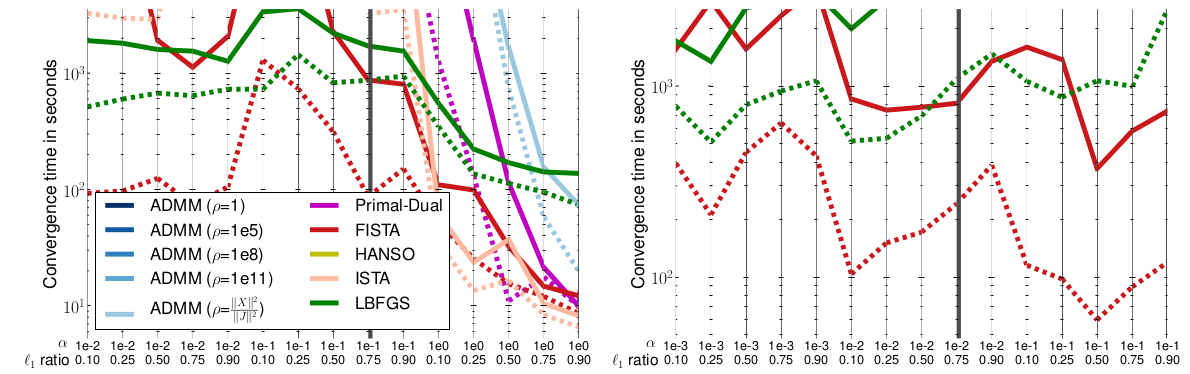
\includegraphics[width=1\linewidth]{figures/solvers_2.png}
   \caption{\textbf{Benchmarking } solvers for TV-$\ell_1$ penalized models. \textbf{Top:} TV-$\ell_1$ penalized Logistic Regression on the visual recognition face-house discrimination task. \textbf{Top Left:} excess energy $E(\B{w}_t ) - E(\B{w}^*)$ as a function of time. \textbf{Top Right:} convergence time of the various solvers for different choice of regularization parameters. Broken lines correspond to a tolerance of
     $10^0$ , whilst full-lines correspond to $10^{-2}$ . The thick vertical line indicates the best model selected by cross-validation. \textbf{Bottom:} TV-$\ell_1$ penalized Least-Squares Regression. \textbf{Bottom Left:} on the visual recognition face-house discrimination task; \textbf{Bottom Right:} on the Mixed gambles dataset. The thick vertical line indicates the best model selected by cross-validation.}
   \label{fig:tvl1bench}
\end{figure}

\label{sec:results}
Here, we present benchmark results for our experiments. Figure
\ref{Fig:HaxbyLR} gives results for the logistic regression run on the
visual recognition dataset: convergence plots of energy as a function of
time show that all methods are asymptotically decreasing. The left part of
Fig. \ref{fig:tvl1bench}
shows the time required to give a convergence
threshold, defined as a given excess energy compared to the lowest energy
achieved by all methods, for different choices of regularization
parameters. Similarly, the right part of Fig. \ref{fig:tvl1bench} shows convergence times
for squared loss on both datasets. For these figures,
each solver was run for a maximum of 1 hour per problem. Solvers that do
not appear on a plot did not converge for the corresponding
tolerance and time budget.

For logistic loss, the most serious contender is
algorithm \ref{Tab:pseudocode_lbfgs}, LBFGS applied on a smooth
surrogate, followed by ADMM, however ADMM performance
varies markedly depending on the choice of $\rho$. For the squared loss
FISTA and algorithm \ref{Tab:pseudocode_lbfgs} are the best performers,
with FISTA achieving a clear lead for the larger mixed-gambles dataset.
Note that in the case of strong regularization the problem is better
conditioned, and first-order methods such as the
primal-dual approach can perform well.

\section{More speed via univariate feature-screening and early-stopping}
In our PRNI 2015 conference paper   \citep{dohmatob2015speeding}, we presented some heuristics for speeding up the overall optimization process: (a) Early-stopping, whereby one  halts
the optimization process when the test score (performance on left-out
data) for the internal cross-validation for model-selection stops
improving, and (b) univariate feature-screening, whereby irrelevant
(non-predictive) voxels are detected and eliminated before the
optimization problem is entered, thus reducing the size of the
problem.

Empirical results with GraphNet on real MRI (Magnetic
Resonance Imaging)
datasets indicated that these heuristics are a win-win strategy, as
they add speed without sacrificing the quality of the predictions
/ classifications.

 \begin{figure}[!htb]
   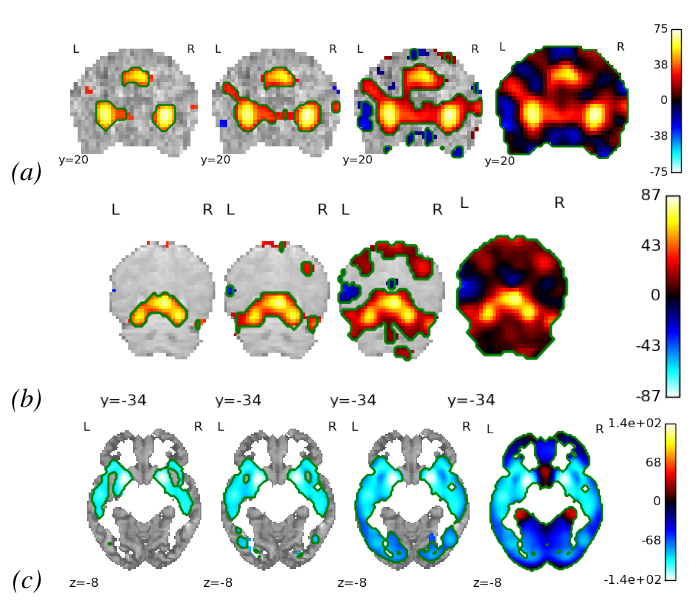
\includegraphics[width=1\linewidth]{figures/screening.png}
\caption{Univariate feature-screening for the
  GraphNet~\citep{hebiri2011,grosenick2013}
  problem \eqref{eq:opt_pb} on
  different datasets.
  % $(\X,\y)$.
  This figure shows spatial maps of
  $\B{X}^T_j\y$, thresholded so that only voxels $j$ with (from left to
  rightmost column)  $|\B{X}^T_j\y| \ge p_{10\%}(|\B{X}^T\y|)$, $|\B{X}^T_j\y| \ge
  p_{20\%}(|\B{X}^T\y|)$, $|\B{X}^T_j\y| \ge p_{50\%}(|\B{X}^T\y|)$, and $|\B{X}^T_j\y|
  \ge p_{100\%}(|\B{X}^T\y|)$ (full-brain) respectively, survive. The
  green contours enclose the elite voxels which are selected by the
  screening procedure at the respective threshold
  levels. \textit{(a)}: Mixed Gambles dataset
   \citep{jimura2012}.%  Remarkably, the geometry of the regions obtained
  % here for the 10th and 20th screening-percentiles match pretty well
  % the results obtained in  \citep{gramfort2013} with their TV-L1
  % penalty. \textit{(b)}: Face vs House contrast of the visual recognition
  % dataset  \citep{haxby2001}. 
  Weights maps obtained for the GraphNet
  model \eqref{eq:opt_pb} with these different
  screening-percentiles are shown in Figure
  \ref{fig:haxby}. \textit{(c)}: OASIS dataset  \citep{marcus2007open}
  with VBM. See Figure \ref{fig:oasis} for weights maps and
  age predictions obtained using these different
  screening-percentiles. % on the GraphNet model \eqref{eq:opt_pb}.
}

\label{fig:screening}
\end{figure}

\subsection{Methods}
%% We will now detail the heuristic techiques for speeding up
%% numerical optimization of GraphNet  \citep{hebiri2011,grosenick2013}
%% model for brain data.


% \paragraph{A note on implementation of the solver.}
One notes that in the case of GraphNet, the penalty term % $J(\w)$
of problem
\eqref{eq:opt_pb}, the $\|\nabla
\w\|^2_2$ sub-term is smooth (i.e differentiable) with
\textit{Lipschitz} gradient, whilst the $\ell_{1}$ term though
nonsmooth, is \textit{proximable}\footnote{That is, there is a
  closed-form analytic expression for its proximal operator.} by means
of the \textit{soft-thesholding} operator  \citep{daubechies2004}.  Thus
problem \eqref{eq:opt_pb} is amenable to the FISTA (Fast Iterative
Shrinkage-Thresholding Algorithm)  \citep{beck09fista}, with a provable
$\mathcal{O}(1/\sqrt{\epsilon})$ convergence rate. Our implementation
of FISTA uses technical recommendations
(line-searching, parametrization, etc.) which were provided in
 \citep{dohmatob2014benchmarking}, in the context of TV-L1
 \citep{baldassarre2012,gramfort2013}. The model parameters $\alpha$ and
$\rho$ in \eqref{eq:opt_pb} are set by \textit{internal}
cross-validation.

%% \paragraph*{(b) Warm-start}
%% The $(\alpha, \rho)$ parameter grid is walked $\rho$-first. For each $\rho$ value encountered, the alphas are walked from largest to smallest value. The largest value is contructed to be the largest value of $\alpha$ for which the optimal solution to problem \eqref{eq:opt_pb} is necessarily zero.

%% We now provide details on the speedup heuristics for speeding up
%% the overall implementation, including model-selection part of it.


\paragraph{Univariate feature-screening.}
%% \textbf{XXX: In a paragraph briefly give a comprehensive overview of
%%   screening algorithms and heuristics from El Ghaoui, upto the more
%%   recent Liu et al!!!}
In machine-learning, feature-screening aims at detecting and
eliminating irrelevant (non-predictive)
features thus reducing the size of the underlying
optimization problem (here problem \eqref{eq:opt_pb}). The general idea
is to compute for each value of the regularization parameter, a
\textit{relevance measure} for each feature, which is then compared with a
threshold (produced by the screening procedure itself). Features which fall short
of this threshold are detected as irrelevant and eliminated. For the
Lasso and similar models (including Group Lasso),
\textit{exact}
screening techniques (i.e, techniques
  which don't mistakenly discard active predictive features) include those developed in
 \citep{elghaoui2010,lee2014exact,liu2014safe,wang2015lasso}. Inexact
screening techniques (e.g  \citep{tibshirani2010strong}) have also been
proposed in the literature.
Our proposed heuristic screening technique is inspired by the
\textit{Marginal screening} technique developed in Algorithm 1 of
 \citep{lee2014exact}, and operates as
follows. The data $(\X,\y)$ are standardized so that $\y$ has unit
variance and zero mean, likewise each row of the design matrix $\X$. To
ensure obtention of a smooth mask, a Gaussian-smoothed version
of $\X$ is used in the screening procedure (but not in the actual model
fit).
For each voxel $j$ (voxels are the features here) the
absolute dot-product $|\B{X}^T_j\y|$ of $\y$ with the $j$th column of
$\X$ is computed.
% This is used as the relevance measure.
For a given screening-percentile
$sp \in [0, 100]$ , the $sp$th percentile value of the
vector $|\B{X}^T\y| := (|\B{X}^T_1\y|, ..., |\B{X}^T_p\y|)$, denoted $p_{sp}(|\B{X}^T\y|)$,
is computed. The case $sp=100$ corresponds to full-brain analysis. 25
means we keep the quarter of the brain made of voxels with the highest
$|\B{X}^T_j\y|$ values, and so on.
% ; this is the threshold.
A brain-mask is then formed containing only those voxels $j$
for which $|\B{X}^T_j\y| \ge p_{sp}(|\B{X}^T\y|)$. Next, this brain-mask is
morphologically eroded
% (to remove isolated small patches)
and then
dilated, to obtain a more structured mask.  Figure
\ref{fig:screening} shows results of applying this screening heuristic
to various datasets, prior to model fitting.

\subsection{Experiments}
We experimented our early-stopping and (separately)
feature-screening heuristics on different MRI datasets.
All experiments were run using a single core of
  a laptop.

\paragraph{Regression.} The OASIS dataset
     \citep{marcus2007open} consists of a
    cross-sectional collection of 416 subjects aged 18 to 96. For each
    subject, 3 or 4 individual T1-weighted MRI scans obtained in
    single scan sessions are included.   A natural regression problem
    for this dataset is to predict the age of a subject from their
    anatomical data. To this end, we segmented the gray-matter from
    the anatomy of each subject (obtained from the T1 images), and
    used the gray-matter maps
    as features for predicting age. We split the 416 subjects into two
    equally-sized and age-balanced groups: a train set and a validation
    set. The GraphNet model  \citep{hebiri2011,grosenick2013} was fitted
    on the train set, with parameters
    ($\alpha$ and $\rho$ in \eqref{eq:opt_pb}) set internally via 8-fold
    cross-validation. The results for this experiment are shown in
    Figure \ref{fig:oasis}.

\paragraph{Classification.} The visual
    recognition dataset  \citep{haxby2001} is a popular block-design
    fMRI dataset from a
    study on face and object representation in human ventral temporal
    cortex.
It consists of 6 subjects with 12 runs per subject. In each run, the
subjects
passively viewed images of eight object categories, grouped
in 24-second blocks separated by intermittent rest periods. This
experiment is a classification task: predicting the object category
$\y$. We use a \textit{One-versus-Rest (OvR)} strategy. The design
matrix $\B{X}$ is made of
time-series from the full-brain mask of $p = 23\,707$ voxels over $n =
216$ TRs, of a single subject (subj1). We divided the 12 runs into 6
runs for training and 6 other runs for
validation. \textit{Leave-one-label-out} cross-validation was used for
selecting the model parameters $(\alpha, \rho)$. The results are
depicted in Figure \ref{fig:haxby}.

\subsection{Results.}
We now summarize and comment the results of the experiments (refer to
section \ref{sec:experiments}).
Figure \ref{fig:oasis} shows the effects of early-stopping heuristic
and feature-screening heuristic on age prediction scores on the OASIS
dataset  \citep{marcus2007open} (416 subjects). We see that in the
internal cross-validation, stopping  the optimization procedure for
fixed $(\alpha, \rho)$ pair of regularization parameters, when test
score increases by $-10^{-2}$ or more is a good heuristic, and does just
as good as running the optimization until numerical convergence. 
 \begin{figure}[!htb]
   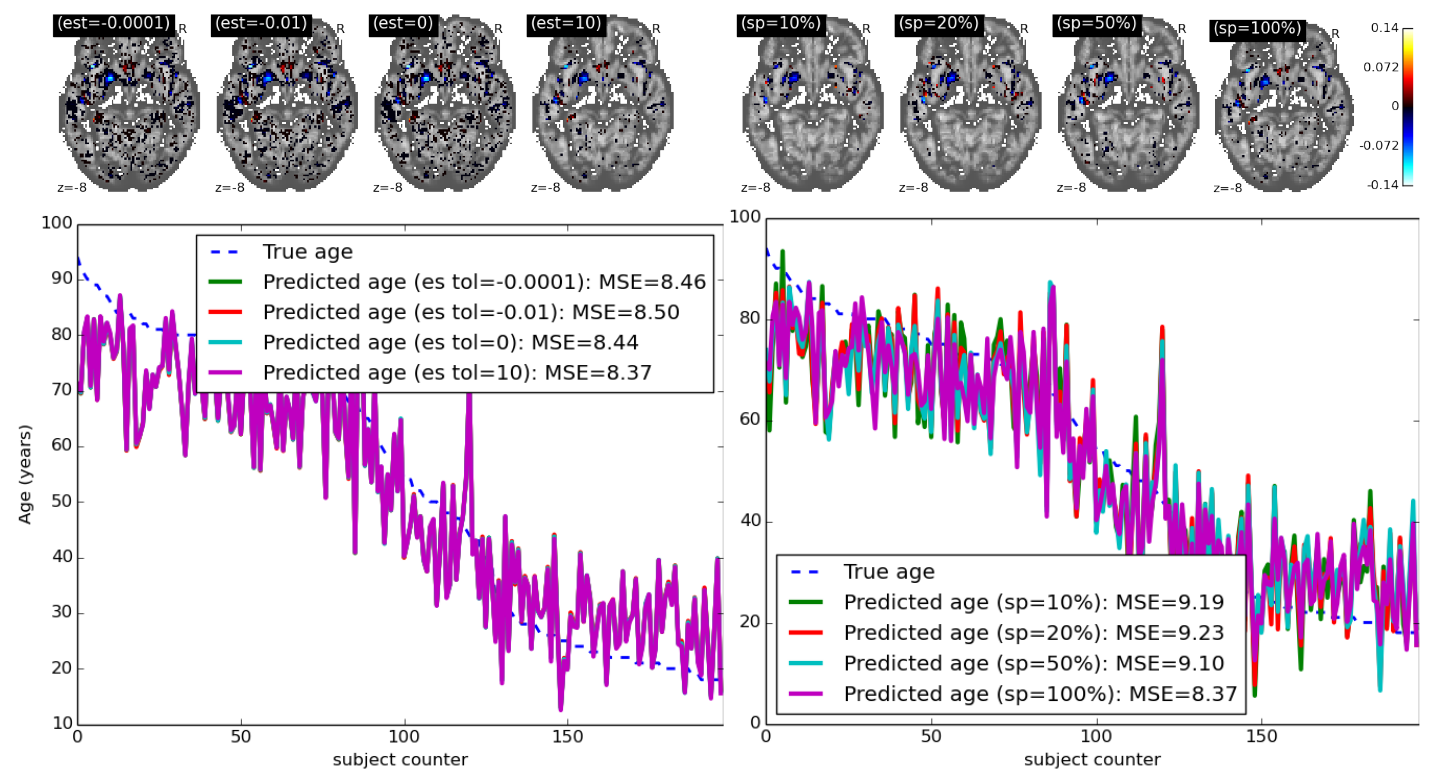
\includegraphics[width=1\linewidth]{figures/screening_weights.png}
  \caption{Predicting age from gray-matter concentration maps from the
    OASIS dataset  \citep{marcus2007open}. \textbf{Top}:
    Weights maps (solutions to problem \eqref{eq:opt_pb}).
% \textbf{N.B}: The long spiky undershoots in the prediction curves
% are indicative of outliers: subjects for which spatial preprocessing
% (tissue segmentation, normalization, etc.) failed.
\textbf{Bottom-left}: Mean Square Error (MSE) in age prediction, for
different subjects of the validation set, for  varying levels of the
early-stopping tolerance (``es tol'' for short), with the
screening-percentile (sp) held constant at 100
(full-brain). \textbf{Bottom-right}: MSE in age prediction, for
varying levels of the screening-percentile (sp).%  \textbf{Running
%   times}: Increasing \textit{est tol} (from $-10^{-4}$ to $10$): \textbf{100.2m, 171.4m, 188.8m, 289.6m}. For
% increasing $sp$ ($10$ to $100$): \textbf{44.2m, 81.3m, 186.5m, 341.3m}
}   
\label{fig:oasis}
\end{figure}
Also (and independently), one gets similar prediction scores using as
little as a fifth of the brain volume ($sp=20$),
compared to using the full-brain ($sp=100$).
Figure \ref{fig:haxby} reports similar results for classification on
the visual recognition dataset  \citep{haxby2001}. Overall, we see from
Figures \ref{fig:haxby} and \ref{fig:oasis} that we can achieve upto
$10$-fold speedup with the proposed heuristics, with very little loss
in accuracy. Also, we see that contiguous groups of bars are roughly flat at the top, with a
    sligh increase from lower to high screening-percentile values. The
    case ``chair vs scramped'' is an exception, where a slightly reverse tendency
    if observed. A possible explanation is that $20$th percentile
    feature-screening already selects the right voxels (quasi-exact
    support recovery), and so including more voxels in the model can only hurt its
    performance...    

 \begin{figure}[!htb]
   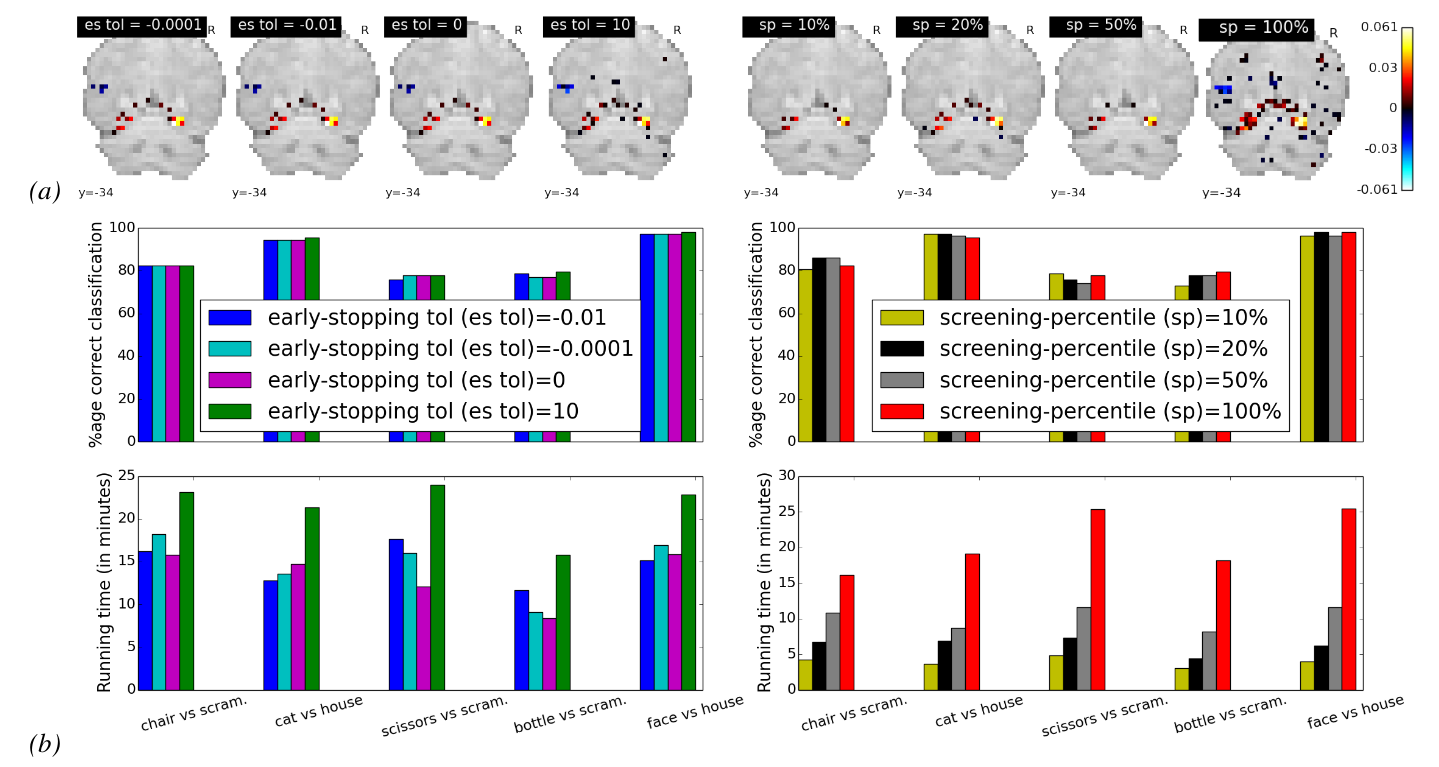
\includegraphics[width=1\linewidth]{figures/screening_weights_haxby.png}
  \caption{Predicting age from gray-matter concentration maps from the
    OASIS dataset  \citep{marcus2007open}. \textbf{Top}:
    Weights maps (solutions to problem \eqref{eq:opt_pb}).
% \textbf{N.B}: The long spiky undershoots in the prediction curves
% are indicative of outliers: subjects for which spatial preprocessing
% (tissue segmentation, normalization, etc.) failed.
\textbf{Bottom-left}: Mean Square Error (MSE) in age prediction, for
different subjects of the validation set, for  varying levels of the
early-stopping tolerance (``es tol'' for short), with the
screening-percentile (sp) held constant at 100
(full-brain). \textbf{Bottom-right}: MSE in age prediction, for
varying levels of the screening-percentile (sp). \textbf{Running
  times}: Increasing \textit{est tol} (from $-10^{-4}$ to $10$): \textbf{100.2m, 171.4m, 188.8m, 289.6m}. For
increasing $sp$ ($10$ to $100$): \textbf{44.2m, 81.3m, 186.5m, 341.3m}}   
  \caption{Visual recognition dataset
     \citep{haxby2001}. \textbf{\textit{(a)}}: Weights maps
    % (maps of
    % regression coefficients $\hat{w}$)
    for the Face vs House contrast,
    for different early-stopping and univariate feature-screening
    thresholds. One can see that the supports of these maps for
    different values of the thresholds are quite similar to cases
    involving  no heuristic at all (the case where est $= 10$ and the
    where case sp $=100\%$).
    \textbf{\textit{(b)}, top-left}: Prediction scores as a function of
    the early-stopping tolerance (est), for different task contrasts.
    \textbf{\textit{(b)}, top-right}: Prediction scores as a function of
    the screening-percentile (sp), for different task contrasts.
    \textbf{\textit{(b)}, bottom-row}: Running times in minutes for the
    different thresholds of the heuristics.
    % As was to be expected, full-brain
    % (sp=100\%) is the most expensive scenario.
  }
  \label{fig:haxby}
\end{figure}
    
 In   \citep{dohmatob2015speeding}, we empirically showed on various
datasets that such screening leads to linear speed-up in the computation
time, while sacrificing prediction / classification power as long as the
screening is not very savage. We also showed that early-stopping the
estimator does not harm the accuracy of the predictions, and can also lead
to considerable (though less systematic speedups).
The result of these numerous ramblings on optimizing the SpaceNet model \eqref{eq:opt_pb} have been implemented as part of the \textit{Nilearn} package   \citep{nilearn}.


% \newthought{We have seen} in Chapter~\ref{chap:stats_fmri} that%  encoding and decoding models take 
% as input  brain activation coefficients (also known as activation patterns or beta-maps). These are usually computed by means of the general linear model (GLM), which
% relies on a \mbox{data-independent} \emph{canonical} form of the hemodynamic response function
% (HRF).


% In this chapter we describe a novel method for the simultaneous estimation of HRF and activation coefficients based on low-rank modeling, forcing the estimated HRF to be equal across events or experimental conditions,
%  yet permitting it to differ across voxels. The estimation of this model leads to
% an optimization problem that we propose to solve with using a
% \mbox{quasi-Newton} method, exploiting fast gradient computations. 
% We compare 10 different HRF modeling methods in terms of encoding and decoding
% score on two different datasets. These results show that the \mbox{R1-GLM} model
% outperforms competing methods in both encoding and decoding
% settings, positioning it as an attractive method both from the points of view
% of accuracy and computational efficiency.

% \hspace{20pt}
% \begin{shaded}
% The contributions developed in this chapter have been published in:
% \begin{itemize}
% \item F. Pedregosa, M. Eickenberg, P. Ciuciu, and B. Thirion, \emph{``Data-driven HRF estimation for encoding and decoding models''} NeuroImage, Volume 104, 1 January 2015, Pages 209-220.

% \item F. Pedregosa, M. Eickenberg, B. Thirion, and A. Gramfort, \emph{“HRF estimation improves sensitivity of fMRI encoding and decoding models”} Proc. 3nd Int. Work. Pattern Recognit. NeuroImaging, 2013.
% \end{itemize}
% \end{shaded}

% \newpage
% \vspace*{\fill}
% \minitoc
% \vspace*{\fill}
% \newpage


% \section{Sparsity and smoothness priors for improved estimation in high dimensions}
% \newthought{Michel et al. 2011, Baldasarre et al. 2012, Gramfort et al. 2013, Abraham et al. 2013, Dohmatob et al. 2014(5), Varoquaux et al. 2016}, ...

% \begin{marginfigure}[4cm]
% \hspace{-20pt}\includegraphics[width=1.2\linewidth]{chapter_3/hrfs_age.pdf}
% \caption{
% 	The HRF can vary substantially between subjects, brain regions and age. In  \citept{colonnese2007development}, the authors studied the evolution of the HRF across age in rats. By comparing fMRI measurements with electrophysiological recordings, they observed two significant trends as age increased: growing amplitude and decreasing time to peak. In the figure, estimated HRF for three groups of rats (with age P13-15 < P20-30< Adult). Source:  \citepp{colonnese2007development}. A comparison of the HRF in human subjects was performed in~ \citepp{badillo2014multi}.
% }
% \end{marginfigure}


% fMRI acquisitions consist of successive brain scans, given in intervals ranging from 1 to 4 seconds. The extraction of time-independent \gls{activation coefficient} from the BOLD time course is commonly done with a model known as Linear General Model
% (GLM)~ \citepp{Friston1995}. While
% this approach has been successfully used in a wide range of studies, it does
% suffer from limitations~ \citepp{Poline2012}. For instance, the GLM commonly
% relies on a \mbox{data-independent} \emph{reference} form of the hemodynamic response function
% (HRF) to estimate the activation coefficient (also known as \emph{canonical HRF}). However it is
% known~ \citepp{Handwerker2004,Badillo2013} that the shape of this response function
% can vary substantially across subjects, age and brain regions. This suggests that an adaptive modeling of this
%  response function should improve the accuracy of subsequent analysis.

% % \emph{feature-extraction} model that extracts 

% % In this section we describe a method that allows to estimate time-independent \gls{activation coefficient} given the BOLD time course. {\blue Feature extraction}. This model is known as the \emph{general linear model}~ \citepp{Friston1995}. In this chapter we describe the main assumptions behind this model: a known form of the hemodynamic response function and the linear-time-invariant property between the BOLD signal and the neural response. 

% % We have seen in Chapter 2 that both encoding and decoding models take as input voxel-wise activation coefficients. These are commonly are computed by means of the General Linear Model
% % (GLM)~ \citepp{Friston1995}. While
% % this approach has been successfully used in a wide range of studies, it does
% % suffer from limitations~ \citepp{Poline2012}. For instance, the GLM commonly
% % relies on a \mbox{data-independent} \emph{reference} form of the hemodynamic response function
% % (HRF) to estimate the activation coefficient (also known as \emph{canonical HRF}). However it is
% % known~ \citepp{Handwerker2004,Badillo2013} that the shape of this response function
% % can vary substantially across subjects, age and brain regions. This suggests that an adaptive modeling of this
% %  response function should improve the accuracy of subsequent analysis.

% To overcome the aforementioned limitation, Finite Impulse Response (FIR) models have been
% proposed within the GLM framework~ \citepp{Dale1999,Glover1999}.
% These models do not assume any particular shape for the HRF and amount to
% estimating a large number of parameters in order to identify it. 
% While the FIR-based modeling makes it possible to estimate the
% activation coefficient and the HRF simultaneously, the increased flexibility
% has a cost. The estimator is less robust and prone to overfitting, i.e. to generalize poorly to unseen data. 
% In general, FIR
% models are most appropriate for studies focused on the characterization of the
% shape of the hemodynamic response, and not for studies that are primarily
% focused on detecting activation~ \citep[Chapter~5]{Poldrack}.

% Several strategies aiming at reducing the number of degrees of freedom of the
% FIR model - and thus at limiting the risk of overfitting - have been proposed.
% One possibility is to constrain the shape of the HRF to be a linear
% combination of a small number of basis functions. A common choice of basis is 
% formed by three elements consisting of a reference HRF as well as its time and dispersion
% derivatives~ \citepp{friston1998nonlinear}, although it is also possible to compute a
% basis set that spans a desired function
% space~ \citepp{Woolrich2004}. More generally, one can also define a parametric
% model of the HRF and estimate the parameters that best fit this
% function~ \citepp{Lindquist2007}. However, in this case the estimated HRF may no longer be a linear function of the input parameters. 

% Sensitivity to noise and overfitting can also be reduced through
% regularization. For example, temporal regularization has been used in the
% smooth FIR ~ \citepp{Goutte2000,Ciuciu2003,Casanova2008} to favor solutions with
% small second order time derivative. These approaches require the setting of
% one or several hyperparameters, at the voxel or potentially at the parcel
% level (if several voxels in a pre-defined parcel are assumed to share some aspects of the HRF time course). Even if efficient techniques such as generalized   
% \mbox{cross-validation}~ \citepp{golub1979generalized} can be used to choose the
% regularization parameters, these methods are inherently more costly than 
% \mbox{basis-constrained} methods. \mbox{Basis-constrained} methods also require
% setting the number of basis elements; however, this parameter is not
% continuous (as in the case of regularized methods), and in practice only few
% values are explored: for example the 3-element basis set formed by a reference HRF
% plus derivatives and the FIR model.  This paper focuses on basis-constrained
% regularization of the HRF to avoid dealing with hyperparameter selection with
% the goal of remaining computationally attractive.  A different approach to
% increase robustness of the estimates consists in linking the estimated HRFs
% across a predefined brain parcel, taking advantage of the spatially dependent nature of
% fMRI~ \citepp{Wang2013}. However, \mbox{hemodynamically-informed}
% parcellations~ \citepp{Chaari2012,Badillo2013a} rely on the computation of 
% a large number of estimations at the voxel or \mbox{sub-parcel} level.
% In this setting, the development of voxel-wise estimation procedures is complementary to the
% development of parcellation methods in that more robust estimation
% methods at the voxel level would naturally translate into more 
% robust parcellation methods. In this thesis we focus on voxel-wise
% estimation methods.


% \paragraph{Contribution}

% In this chapter we have described a method for the simultaneous estimation of HRF and activation coefficients based on low-rank modeling. While the assumptions of this model are not novel (cf.~ \citepp{Makni2008,vincent2010spatially,Degras2014}), the formulation of this model as a least squares problem with a rank-one constraint is a novel contribution. This formulation allows to efficiently solve the problem using gradient-based methods.
% Finally, we evaluate the proposed model on three publicly available datasets. 

% % {\blue With respect to the work published in ~ \citepp{Pedregosa2015209}, we have included in this chapter the results on a new datasets and examined the gain obtained by this model across different regions of the brain}.

% \clearpage
\bibliographystyle{plainnat}
\bibliography{bib_all}
